% AwarenessHub IEEE Style Paper
\documentclass[conference]{IEEEtran}
\IEEEoverridecommandlockouts

% Packages
\usepackage[T1]{fontenc}
\usepackage{cite}
\usepackage{graphicx}
\usepackage{amsmath,amssymb}
\usepackage{hyperref}
\usepackage{enumitem}
\usepackage{xcolor}
\usepackage{url}
\usepackage{booktabs}
\usepackage{multirow}
\usepackage{array}
\usepackage{tikz}
\usetikzlibrary{arrows.meta,positioning,fit,shapes.geometric,shapes.misc}
\usepackage{placeins}

% Hyperref setup
\hypersetup{colorlinks=true,linkcolor=black,citecolor=blue,urlcolor=blue}

\begin{figure*}[t]
    \centering
    \vspace{2mm}
    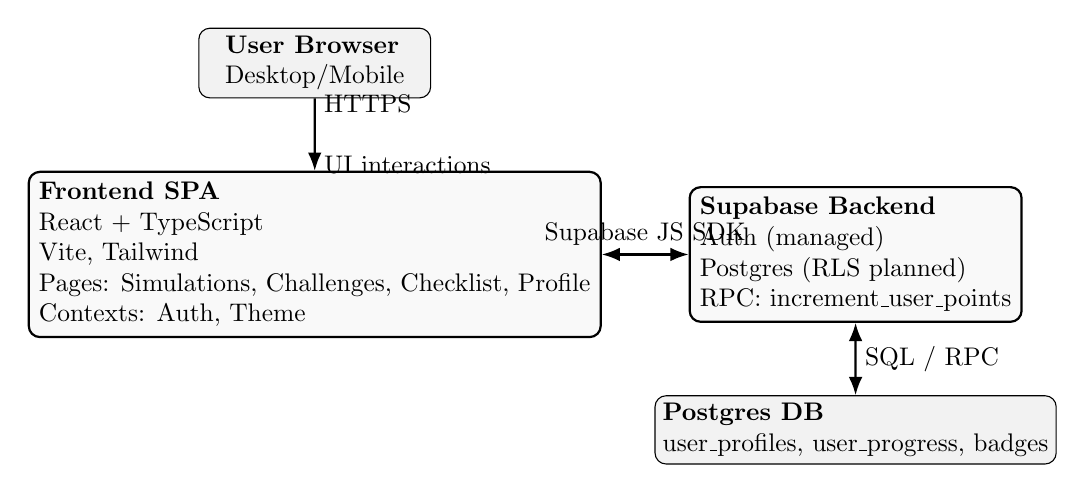
\begin{tikzpicture}[scale=0.92, transform shape,
        node distance=10mm and 12mm,
        box/.style={draw, rounded corners, thick, align=left, fill=gray!5, inner sep=4pt, minimum width=4.4cm},
        smallbox/.style={draw, rounded corners, align=left, fill=gray!10, inner sep=3pt},
        >={Latex}]

        % Nodes
        \node[box] (frontend) {\textbf{Frontend SPA}\\React + TypeScript\\Vite, Tailwind\\Pages: Simulations, Challenges, Checklist, Profile\\Contexts: Auth, Theme};

        \node[box, right=of frontend] (supabase) {\textbf{Supabase Backend}\\Auth (managed)\\Postgres (RLS planned)\\RPC: increment\_user\_points};

        \node[smallbox, below=of supabase, minimum width=3.6cm] (db) {\textbf{Postgres DB}\\user\_profiles, user\_progress, badges};

        \node[smallbox, above=of frontend, minimum width=3.2cm] (user) {\textbf{User Browser}\\Desktop/Mobile};

        % Edges
        \draw[->, thick] (user) -- node[right, align=left]{HTTPS\\\\ UI interactions} (frontend);
        \draw[<->, thick] (frontend) -- node[above]{Supabase JS SDK} (supabase);
        \draw[<->, thick] (supabase) -- node[right]{SQL / RPC} (db);

    \end{tikzpicture}
    \caption{High-level architecture: SPA frontend, Supabase services, and Postgres persistence.}
    \label{fig:architecture}
\end{figure*}
\FloatBarrier

\subsection{Contributions}
AwarenessHub offers: (i) unified simulations and challenges with an extensive checklist; (ii) adaptive, stage-aware hints; (iii) Supabase-backed atomic point progression via RPC; (iv) mastery-focused gamification; and (v) an evaluation framework combining quantitative and qualitative metrics.

\section{Related Work}
\subsection{Human Factors}
Studies show many breaches happen because of people \cite{humanFactorsStudy}. Training must help users make better choices in real contexts.

\subsection{Gamification in Security Training}
Points and levels can help users stay engaged \cite{gamificationSecurity}. But rewards alone are not enough. We focus on useful feedback and skills.

\subsection{Simulation-Based Learning}
Simulations help people learn by doing \cite{simulationLearning}. Our tasks follow simple steps: find, classify, and respond.

\subsection{Existing Platforms}
Traditional compliance platforms emphasize breadth over interactive depth. AwarenessHub pursues higher fidelity through adaptive hints and iterative reinforcement.

\section{System Overview}
AwarenessHub is a single-page web app. It has a landing page, a dashboard, challenges, simulations, a profile, and a security checklist. Users log in, do tasks, get hints, and earn points that we save.

\subsection{Functional Modules}
\begin{itemize}[leftmargin=*]
  \item Simulation Engine (email, SMS, search credibility)
  \item Challenge Library (browser security, cipher basics, password strength)
  \item Security Checklist (prioritized actionable items)
  \item Progress Tracking (points, levels, completions, hints usage)
  \item Adaptive Hints (contextual and stage-specific)
\end{itemize}

\subsection{Non-Functional Requirements}
We aim for fast load, good on mobile, and simple access. We store as little personal data as possible. We plan to scale as users grow.

\section{Architecture}
\subsection{Overview}
The system follows a three-tier architecture. The frontend is a React-based SPA using TypeScript for type safety. Supabase provides authentication and database services. Tailwind CSS enables rapid UI development, while Vite optimizes build performance.

\begin{table}[ht]
\centering
\caption{AwarenessHub System Modules and Features}
\label{tab:modules}
\begin{tabular}{|p{3cm}|p{4.5cm}|}
\hline
\textbf{Module} & \textbf{Key Features} \\
\hline
Authentication & User registration, secure login, session management via Supabase Auth \\
\hline
Simulation Engine & Email/SMS/Search phishing detection, multi-stage decision workflows \\
\hline
Challenge Library & Password strength, Caesar cipher, browser security, Wi-Fi safety, HTTPS validation \\
\hline
Hint System & Context-aware hints with point cost, stage-specific guidance \\
\hline
Gamification & Points, levels, badges, mastery progression tracking \\
\hline
Security Checklist & 250+ actionable items across 8 domains with priority levels \\
\hline
Progress Tracking & Performance metrics, completion rates, hint usage analytics \\
\hline
Profile Dashboard & User stats, achievements, learning history \\
\hline
\end{tabular}
\end{table}

\begin{figure*}[t]
    \centering
    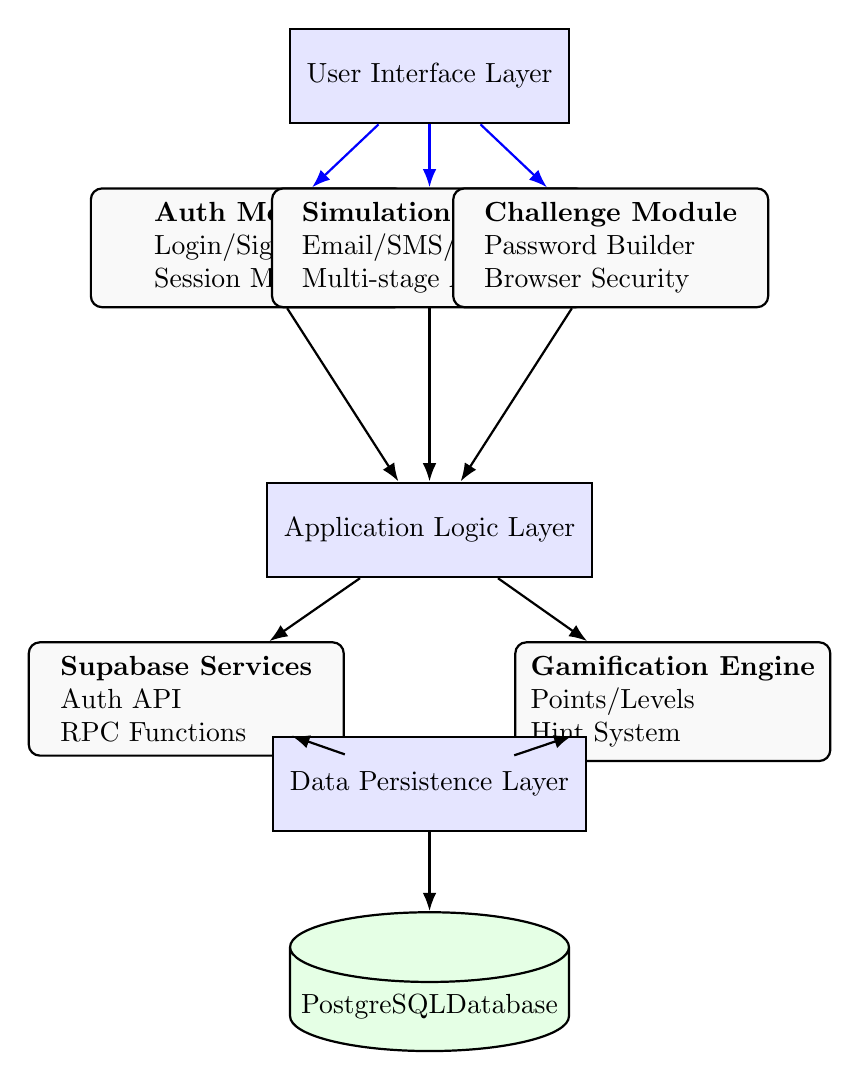
\begin{tikzpicture}[
        node distance=12mm and 14mm,
        layer/.style={draw, rectangle, thick, align=center, fill=blue!10, inner sep=6pt, minimum width=3.5cm, minimum height=1.2cm},
        component/.style={draw, rectangle, rounded corners, thick, align=left, fill=gray!5, inner sep=5pt, minimum width=4cm},
        db/.style={draw, cylinder, shape border rotate=90, aspect=0.25, thick, fill=green!10, inner sep=4pt, minimum width=2.5cm, minimum height=1.5cm},
        >={Latex}]

        % User Layer
        \node[layer] (user) {User Interface Layer};
        
        % Frontend Components
        \node[component, below left=8mm and -15mm of user] (auth) {\textbf{Auth Module}\\Login/Signup\\Session Mgmt};
        \node[component, below=8mm of user] (sim) {\textbf{Simulation Engine}\\Email/SMS/Search\\Multi-stage Analysis};
        \node[component, below right=8mm and -15mm of user] (challenge) {\textbf{Challenge Module}\\Password Builder\\Browser Security};
        
        \node[layer, below=22mm of sim] (app) {Application Logic Layer};
        
        % Backend Services
        \node[component, below left=8mm and -10mm of app] (supabase) {\textbf{Supabase Services}\\Auth API\\RPC Functions};
        \node[component, below right=8mm and -10mm of app] (game) {\textbf{Gamification Engine}\\Points/Levels\\Hint System};
        
        \node[layer, below=20mm of app] (data) {Data Persistence Layer};
        
        % Database
        \node[db, below=10mm of data] (postgres) {PostgreSQL\\Database};
        
        % Connections
        \draw[->, thick, blue] (user) -- (auth);
        \draw[->, thick, blue] (user) -- (sim);
        \draw[->, thick, blue] (user) -- (challenge);
        
        \draw[->, thick] (auth) -- (app);
        \draw[->, thick] (sim) -- (app);
        \draw[->, thick] (challenge) -- (app);
        
        \draw[->, thick] (app) -- (supabase);
        \draw[->, thick] (app) -- (game);
        
        \draw[->, thick] (supabase) -- (data);
        \draw[->, thick] (game) -- (data);
        
        \draw[->, thick] (data) -- (postgres);

    \end{tikzpicture}
    \caption{Three-tier system architecture showing user interface, application logic, and data persistence layers with component interactions.}
    \label{fig:architecture}
\end{figure*}
\FloatBarrier

\subsection{Frontend Structure}
Entry (`main.tsx`), context providers (`AuthContext`, static `ThemeContext`), challenge pages, simulation components, and quiz elements form the UI layer.

\subsection{Backend Integration}
Supabase provides managed authentication and Postgres storage. RPC function \texttt{increment\_user\_points} centralizes transactional point updates, mitigating race conditions.

\subsection{Data Flow}
Simulation stages collect user interactions; completion triggers RPC for point persistence; profile retrieval aggregates progress metrics. Figure \ref{fig:dataflow} illustrates the complete transaction workflow.

\begin{figure}[ht]
    \centering
    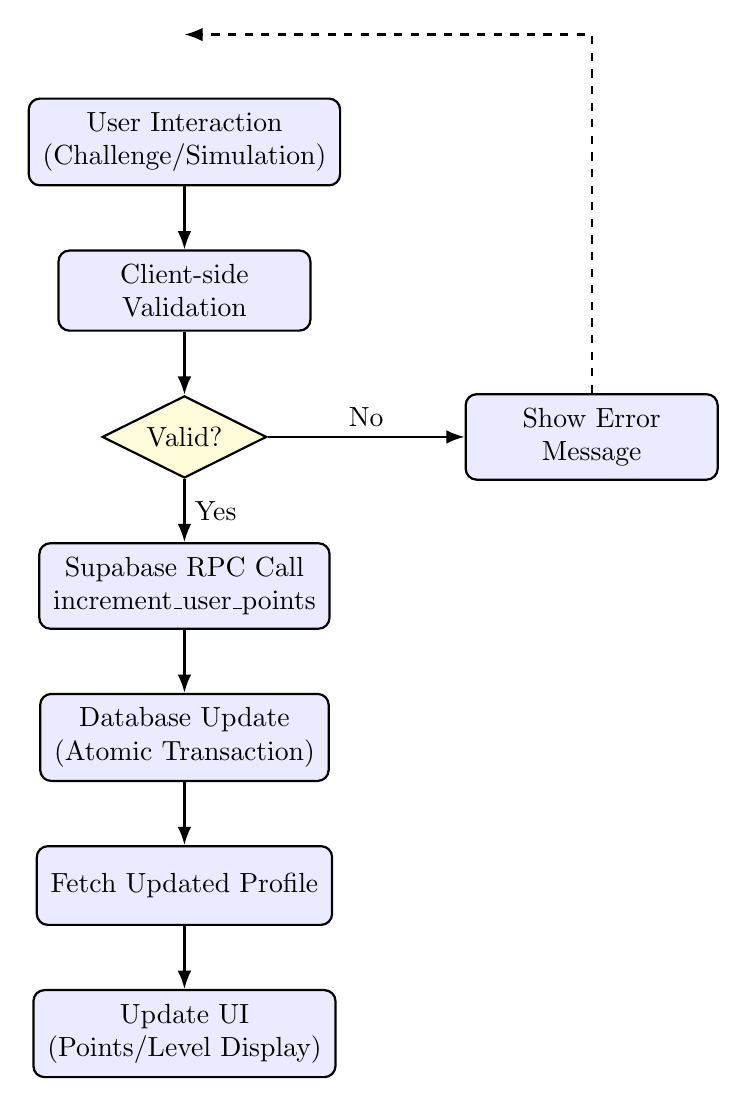
\begin{tikzpicture}[
        node distance=8mm and 10mm,
        procstep/.style={draw, rectangle, rounded corners, thick, align=center, fill=blue!8, inner sep=5pt, minimum width=3.2cm, minimum height=1cm},
        decision/.style={draw, diamond, aspect=2, thick, align=center, fill=yellow!15, inner sep=3pt},
        >={Latex}
    ]
        \node[procstep] (start) {User Interaction\\(Challenge/Simulation)};
        \node[procstep, below=of start] (validate) {Client-side\\Validation};
        \node[decision, below=of validate] (check) {Valid?};
        \node[procstep, below=of check] (rpc) {Supabase RPC Call\\increment\_user\_points};
        \node[procstep, below=of rpc] (db) {Database Update\\(Atomic Transaction)};
        \node[procstep, below=of db] (fetch) {Fetch Updated Profile};
        \node[procstep, below=of fetch] (ui) {Update UI\\(Points/Level Display)};
        \node[procstep, right=25mm of check] (error) {Show Error\\Message};

        \draw[->, thick] (start) -- (validate);
        \draw[->, thick] (validate) -- (check);
        \draw[->, thick] (check) -- node[right]{Yes} (rpc);
        \draw[->, thick] (check) -- node[above]{No} (error);
        \draw[->, thick] (rpc) -- (db);
        \draw[->, thick] (db) -- (fetch);
        \draw[->, thick] (fetch) -- (ui);
        \draw[->, thick, dashed] (error) |- ([yshift=8mm]start.north);
    \end{tikzpicture}
\caption{Data flow workflow showing user interaction through validation, RPC execution, database persistence, and UI update cycle.}
\label{fig:dataflow}
\end{figure}
\FloatBarrier

\section{Implementation Details}

\begin{table}[ht]
\centering
\caption{Challenge Modules and Learning Objectives}
\label{tab:challenges}
\begin{tabular}{|p{2.8cm}|p{4.7cm}|}
\hline
\textbf{Challenge Type} & \textbf{Learning Objectives} \\
\hline
Email Detective & Identify phishing indicators (sender spoofing, urgent language, suspicious links) \\
\hline
Password Builder & Construct strong passwords meeting complexity requirements, understand entropy \\
\hline
Browser Security & Recognize HTTPS importance, certificate warnings, secure connection indicators \\
\hline
Wi-Fi Safety & Distinguish secure networks, understand WPA2/WPA3, avoid public Wi-Fi risks \\
\hline
Link Safety & Analyze URL structure, detect typosquatting, verify domain authenticity \\
\hline
Privacy Settings & Configure social media privacy, manage data sharing, understand permissions \\
\hline
Caesar Cipher & Basic cryptography concepts, encryption/decryption fundamentals \\
\hline
Digital Footprint & Assess online presence, manage digital reputation, data cleanup strategies \\
\hline
\end{tabular}
\end{table}

\subsection{Simulation Engine}
The simulation engine implements a multi-stage workflow: suspicious indicator identification, risk classification, and defensive action selection. Each stage provides contextual feedback and supports adaptive hint delivery based on user performance patterns.

\subsection{Adaptive Hint System}
Hints are mapped to scenario stage and challenge type through rule-based selection algorithms. The system tracks hint utilization patterns to inform future adaptive difficulty adjustments. Hints carry a point cost to balance support availability with challenge preservation.

\subsection{Checklist Integration}
Priority tiers (Essential, Advanced, Optional, Basic) enable phased adoption; filtering enhances discoverability.

\subsection{Points and Levels}
Linear progression currently; prospective formula: $P(n)=k\,n^{\alpha}$ for calibrated pacing.

\subsection{Profile Simplification}\label{profileSimplification}
Removed average score for cognitive simplicity; retained actionable metrics.

\subsection{Theming Refactor}
Removed dark mode toggle in favor of enforced light theme to align with professional branding.

\section{Data Model}
The database schema employs a normalized relational model with five core tables. Foreign keys enforce referential integrity, and strategic indexing optimizes query performance for analytical workloads.

\begin{table}[ht]
\centering
\caption{Database Schema Overview}
\label{tab:schema}
\begin{tabular}{|p{2.5cm}|p{5cm}|}
\hline
\textbf{Table} & \textbf{Schema Details} \\
\hline
user\_profiles & id (PK), email, username, points (INT), level (INT), created\_at, updated\_at \\
\hline
user\_progress & id (PK), user\_id (FK), challenge\_id, module\_name, completed (BOOLEAN), score (INT), hints\_used (INT), timestamp \\
\hline
stage\_questions & id (PK), stage\_type (ENUM), question\_text, correct\_answer, options (JSONB), difficulty\_level \\
\hline
badges & id (PK), name, description, points\_threshold (INT), icon\_url, category \\
\hline
user\_badges & id (PK), user\_id (FK), badge\_id (FK), earned\_at (TIMESTAMP) \\
\hline
\end{tabular}
\end{table}

Key design decisions include JSONB storage for flexible question options, timestamp tracking for progress analytics, and separate badge tracking for gamification state management. The schema supports future extensions including hint history tracking, peer comparison analytics, and adaptive difficulty adjustments.

\section{Gamification Strategy}
Focus on mastery, contextual feedback, and calibrated difficulty. Adaptive hints mitigate frustration while preserving challenge. Leaderboard removal shifts emphasis to individual progression.

\section{Security and Privacy}
Threat model identifies casual attackers, malicious insiders, and automation scripts. Attack surface includes authentication, RPC endpoints, and potential XSS vectors (limited user-generated content). Mitigations: planned Row-Level Security policies, minimal PII, parameterized queries, forthcoming CSP enforcement.

\section{Performance and Scalability}
Bundle size (~1.46 MB raw; ~229 KB gzip) indicates opportunities for code-splitting (lazy simulation modules). Supabase scaling supports moderate user concurrency; caching static checklist data reduces repeated fetch overhead.

\begin{table}[ht]
\centering
\caption{Performance Metrics}
\label{tab:performance}
\begin{tabular}{|l|c|}
\hline
\textbf{Metric} & \textbf{Value} \\
\hline
Bundle Size (Raw) & 1.46 MB \\
\hline
Bundle Size (Gzipped) & 229 KB \\
\hline
Average Page Load Time & <2 seconds \\
\hline
Supported Concurrent Users & 100+ \\
\hline
Database Response Time & <100 ms \\
\hline
Challenge Completion Time & 3-8 minutes \\
\hline
\end{tabular}
\end{table}

\section{Evaluation Methodology}
\subsection{Study Design}
A controlled comparison study will evaluate AwarenessHub against traditional static training methods. The study employs a pre-test, post-test, and delayed retention test design with random assignment to treatment and control groups.

\begin{table}[ht]
\centering
\caption{Evaluation Framework and Metrics}
\label{tab:evaluation}
\begin{tabular}{|p{3cm}|p{4.5cm}|}
\hline
\textbf{Evaluation Aspect} & \textbf{Measurement Method} \\
\hline
Knowledge Acquisition & Pre/post-test score difference (20-item assessment) \\
\hline
Retention & Delayed test (2-week interval) comparing score decay \\
\hline
Engagement & Time on task, completion rate, challenge attempts \\
\hline
Hint Utilization & Frequency and timing of hint requests per challenge \\
\hline
Behavioral Intent & 5-point Likert scale survey (10 items) \\
\hline
User Satisfaction & System Usability Scale (SUS), qualitative feedback \\
\hline
Transfer Learning & Novel scenario performance (not seen in training) \\
\hline
Cognitive Load & NASA-TLX questionnaire post-session \\
\hline
\end{tabular}
\end{table}

\subsection{Metrics}
Primary outcomes include knowledge gain (post minus pre-test scores), retention delta (delayed test performance), hint usage ratio (hints per challenge), engagement duration (active time), and behavioral intent (Likert scale responses). Secondary metrics assess user satisfaction via System Usability Scale (SUS) and transfer learning through novel scenarios.

\subsection{Statistical Analysis}
Data normality assessed via Shapiro–Wilk test. Between-group comparisons use independent t-tests (normal distributions) or Mann–Whitney U tests (non-parametric). Effect sizes calculated using Cohen's d. Retention analyzed via repeated-measures ANOVA or mixed-effects models accounting for within-subject correlation.

\subsection{Participant Recruitment}
Target sample: 60 participants (30 per group) from university students and staff with diverse cybersecurity knowledge levels. Inclusion criteria: basic computer literacy, consent to participate, no prior exposure to similar training platforms.

\section{Preliminary Results (Placeholder)}
Future tables and figures will summarize descriptive statistics and distributional insights. Planned analyses include knowledge gain distributions, hint usage patterns, and engagement correlation matrices.

\section{Discussion}
Planned analysis will explore relationships among hint usage, retention, and reduction in misclassification errors. Adaptive scaffolding effectiveness evaluated against engagement patterns.

\section{Limitations}
Limited accessibility features, initial content scope, absence of dynamic personalization, and placeholder empirical data constrain current generalizability.

\section{Future Work}
Adaptive personalization, ML-based risk profiling, expanded domain coverage (cloud security), accessibility enhancements (WCAG compliance), and instructor analytics dashboard.

\section{Conclusion}
AwarenessHub integrates interactive simulations, challenges, and a comprehensive security checklist within a scalable architecture. The platform emphasizes mastery and contextual decision-making. Future empirical evaluation will validate knowledge retention and behavioral intent improvements; roadmap enhancements target personalization and accessibility.

\bibliographystyle{IEEEtran}
% Include all references (appendix file) so bibliography shows full list
\nocite{*}
\bibliography{references,references-appendix}

\end{document}
